%                                                                 aa.dem
% AA vers. 9.1, LaTeX class for Astronomy & Astrophysics
% demonstration file
%                                                       (c) EDP Sciences
%-----------------------------------------------------------------------
%
%\documentclass[referee]{aa} % for a referee version
%\documentclass[onecolumn]{aa} % for a paper on 1 column  
%\documentclass[longauth]{aa} % for the long lists of affiliations 
%\documentclass[letter]{aa} % for the letters 
%\documentclass[bibyear]{aa} % if the references are not structured 
%                              according to the author-year natbib style

%
\documentclass{aa}  

%
\usepackage{graphicx}
\usepackage{float}
% \usepackage{algorithmic}
\usepackage[lined,ruled,linesnumbered]{algorithm2e}
%%%%%%%%%%%%%%%%%%%%%%%%%%%%%%%%%%%%%%%%
\usepackage{txfonts}
%%%%%%%%%%%%%%%%%%%%%%%%%%%%%%%%%%%%%%%%
%\usepackage[options]{hyperref}
% To add links in your PDF file, use the package "hyperref"
% with options according to your LaTeX or PDFLaTeX drivers.
%
\begin{document} 


   \title{Tunable Kernel-Nulling for direct detection of exoplanets}

   \subtitle{1. Calibration and performance}

   \author{V. Foriel\inst{1},
            F. Martinache\inst{1},
            D. Mary\inst{1}
            \and
            R. Laugier\inst{2}
          }

   \institute{Université Côte d’Azur, Observatoire de la Côte d’Azur Nice, CNRS, Laboratoire Lagrange, Nice, France
         \and
            KU Leuven university, Leuven, Belgium
             }

   \date{Received ---; accepted ---}

% \abstract{}{}{}{}{} 
% 5 {} token are mandatory
 
  \abstract
  % context heading (optional)
  % {} leave it empty if necessary  
   {Lorem ipsum}
  % aims heading (mandatory)
   {Lorem ipsum}
  % methods heading (mandatory)
   {Lorem ipsum}
  % results heading (mandatory)
   {Lorem ipsum}
  % conclusions heading (optional), leave it empty if necessary 
   {Lorem ipsum}

   \keywords{Lorem ipsum}

   \maketitle
%
%-------------------------------------------------------------------

\section{Introduction}

    \begin{enumerate}
        \item Nulling interferometry
        \item Kernel nulling
        \item Integrated optics \& phase shifters
    \end{enumerate}

%--------------------------------------------------------------------

\section{Materials and methods}

    \begin{enumerate}
        \item VLTI/ASGARD (/NOTT?)
        \item Integrated optics \& phase shifters
        \item Studied architecture
        \item Observation conditions (Vegga-like star, noise etc.)
        \item Calibration methods (Fig \ref{fig:perturbed_phases} \& \ref{fig:calibrated_phases})
        \subitem Genertic Algorithm
        \subitem Input obstruction
        \subitem Machine Leaning?
    \end{enumerate}

    \begin{figure}[H]
        \begin{center}
        \begin{tabular}{c}
        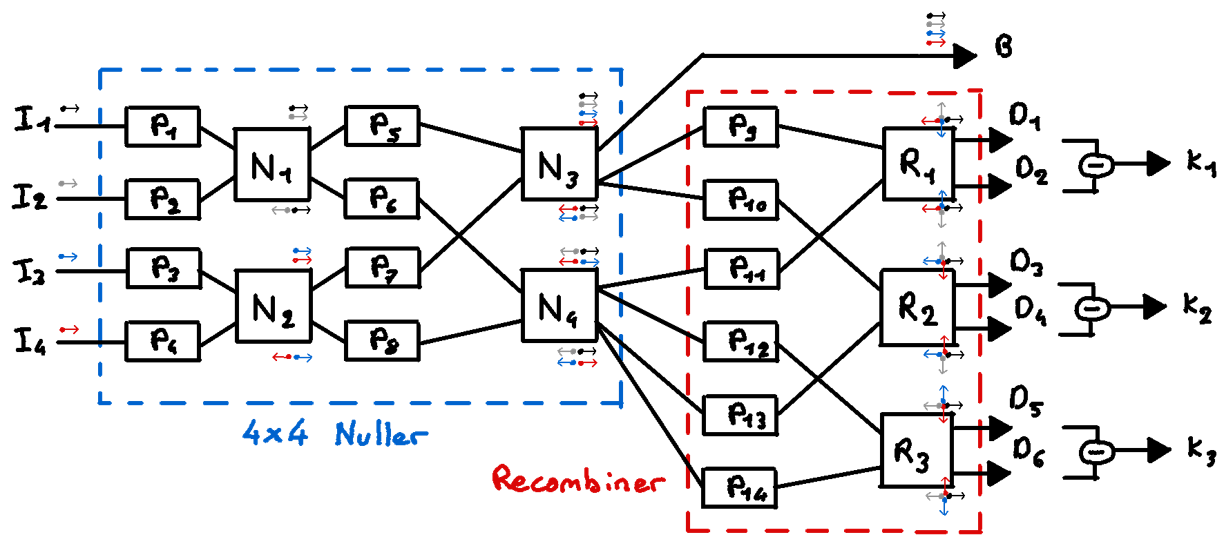
\includegraphics[height=3.5cm]{img/scheme.png}
        \end{tabular}
        \end{center}
        \caption[architecture] 
        { \label{fig:architecture} 
        Studied architecture}
    \end{figure}

    \subsection{Algorithms}
        \subsubsection{Genetic}
            Le premier algorithme à avoir été mis au point repose sur le principe d'algorithme génétique déterministe. On définit une métrique de performance $M$, qui va ici correspondre à la profondeur du kernel-null, puis on cherche à l'optimiser en faisant introduisant successivement une variation de phase $\Delta \phi$ sur chacun des retardateurs $P_i$.

            Le processus d'optimisation se fait en utilisant une source ponctuelle qui simule une étoile seule. Le but est alors d'annuler son signal. Toutefois, étant donné que les Kernels sont construit via la différence de deux sorties sombres, il est possible d'obtenir de très bon kernel-nulls sans pour autant avoir bien annulé la lumière de l'étoile. Pour palier à ce problème, on définit alors deux métriques, l'une mesurant la profondeur du kernel-null $M_K$, l'autre l'intensité obtenue sur la sortie brillante du coposant $M_B$. Ainsi, on a :

            \begin{equation}
                M_K = \left||D_1|^2 - |D_2|^2\right| + \left||D_3|^2 - |D_4|^2\right| + \left||D_5|^2 - |D_6|^2\right|
            \end{equation}

            \begin{equation}
                M_B = |B|^2
            \end{equation}
            
            Au regard de l'architecture de notre composant, on peut alors associer la métrique $M_B$ à chacun des retardateurs qui influent sur la sortie brillante, soit $P_{1 \rightarrow 5}$ ainsi que $P_7$. L'ensemble des autres retardateurs sont alors associé à la métrique $M_K$.

            L'algorithme génétique se construit alors de la façon suivante :

            \begin{enumerate}
                \item Initialisation : on initialise les phases de chacun des retardateurs à 0
                \item Mutation : on introduit une variation de phase $+ \Delta \phi$ puis de $- \Delta \phi$ successivement sur chaque retardateur $P_i$ (toujours dans le même ordre).
                \item Sélection : on conserve la configuration qui a le plus amélioré la métrique associé à ce retardateur.
                    \subitem Si $i \in [1, 5] \cup 7$, on conserve la variation qui a le plus augmenté la métrique $M_B$ (redirection de l'ensemble du flux de létoile sur la sortie brillante)
                    \subitem Si $i \in 6 \cup [8, 14]$, on conserve la variation qui a le plus réduit la métrique $M_K$ (symétrisation des sorties sombres pour creuser la profondeur des kernel-nulls)
                \item Convergence : on répète les étapes 2 et 3 en réduisant à chaque fois la valeur de $\Delta \phi$ d'un facteur $\beta \in [0.5,1[$. Un facteur $\beta$ proche de $1$ permet une convergeance lente mais plus précise, là où un facteur $\beta = 0.5$ donnera la meilleur vitesse de convergeance mais peut régulièrement manquer de précision.
                \item Point d'arrêt : on s'arrête lorsque la variation de phase $\Delta \phi$ introduite est inférieur à l'incertitude sur la phase injectée, qui doit être déterminé via une caractérisation préalable des retardateurs de phase.
            \end{enumerate}
            
            % \IncMargin{1em}
            \begin{algorithm}
            %\SetKwData{Left}{left}\SetKwData{This}{this}\SetKwData{Up}{up}
            %\SetKwFunction{Union}{Union}\SetKwFunction{FindCompress}{FindCompress}
            \SetKwInOut{Input}{Inputs}\SetKwInOut{Output}{Output}
            \Input{$\epsilon, \beta$}
            \BlankLine
            \Output{\vec{P}}
            \BlankLine
            
            $\vec P \leftarrow \vec 0$;\\
            $\vec \psi \leftarrow \vec 1 \times \frac{1}{\sqrt{4}}$;\\
            $\vec PM_K \leftarrow [1,5] \cup [7]$; $\vec PM_B \leftarrow [6] \cup [8,14]$;\\
            
            \caption{Genetic algorithm}
            \label{genetic}
            \end{algorithm}
            \DecMargin{1em}

            Cet algorithme a pour avantages d'être très facile à adapter à d'autres architectures de Kernel-Nuller et ne fait intervenir aucune pièce mobile durant le processus de calibration ce qui permet une calibration automatisée et rapide. En revanche, il souffre d'une limitation lié au bruit de photon. En effet, les retards de phase à injecter sur les retardateurs des couches proches des sorties dépendent des retards de phase injectés sur les couches précédentes. Ainsi, la calibration des dernier retardateurs ne peut se faire finament qu'une foit les premiers retardateurs calibrés, ce qui a pour conséquence d'avoir très peu de flux sur les sorties sombres lors de la calibration et ainsi d'augmenter la sensibilité au bruit de photon. Numériquement, même en tenant compte du bruit de photon, il est toutefois possible d'atteindre des profondeur de kernel-null de l'ordre de $10^{-8}$. [RAJOUTER LES RESULTATS EN LABO]. Un autre défaut de cet algorithme réside dans le fait que la convergeance peut être sous-optimale. La fréquence de ce genre de cas décroit lorsque $\beta$ est proche de 1, ce qui implique une convergeance plus lente.

            \begin{figure}[H]
                \begin{center}
                \begin{tabular}{c}
                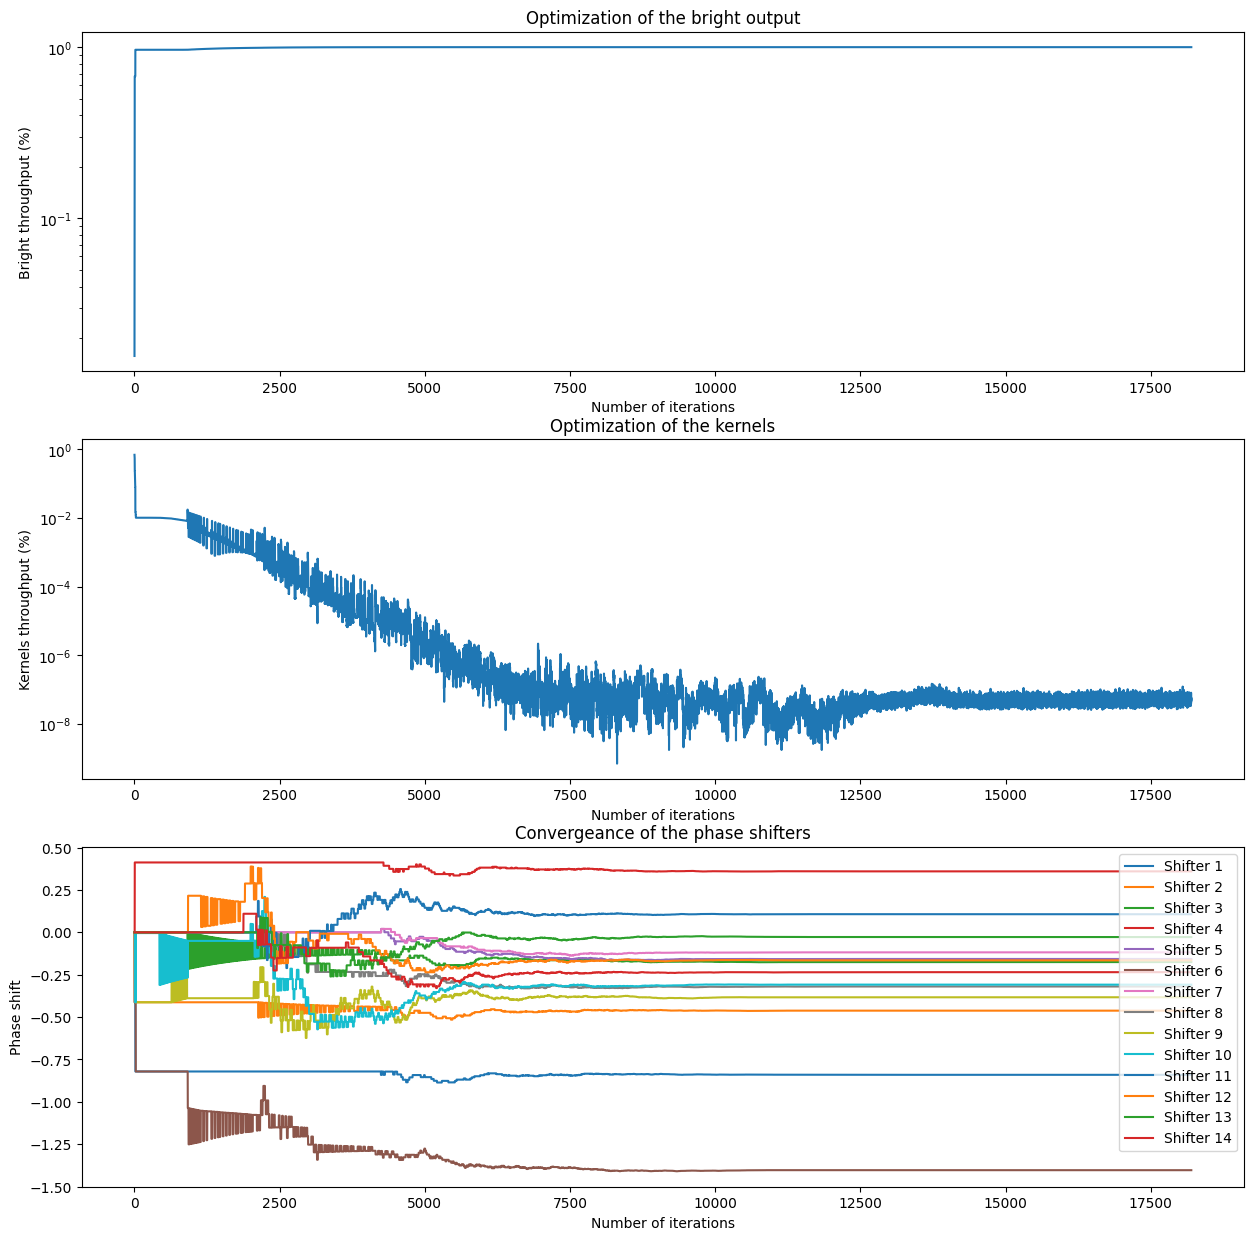
\includegraphics[height=7cm]{img/calibration_genetic.png}
                \end{tabular}
                \end{center}
                \caption[calibration_genetic] 
                { \label{fig:calibration_genetic} 
                Calibration using genetic algorithm [AJOUTER DESCRIPTION]}
            \end{figure}

        \subsubsection{Input obstruction}
            Afin de palier aux limitations de l'algorithme génétique, une autre méthode de calibration a été mise en place. Cette méthode repose sur le principe d'obstruction des entrées du composant. On injecte toujours une source ponctuelle dans le composant mais l'on obstrue cette fois 2 de ses entrées. On s'intéresse alors à l'une de ses sorties dont la fontion de transfert se retrouve grandement simplifiée, au point de n'avoir plus qu'un seul paramètre (retardateur de phase) influencant sur cette sortie.

            L'algorithme se construit alors de la façon suivante :

            \begin{enumerate}
                \item On obstrue les entrées 3 et 4 puis on chercher à maximiser la sortie brillante. Etant donné qu'on est insensible à la phase globale, on peut utiliser la phase du champ élctrique de la première entrée comme phase de référence. Ainsi, la sortie brillante peut être maximisée en jouant uniquement sur le retardateur $P_2$.
                \item On obstrue les entrées 1 et 2 puis on cherche à maximiser la sortie brillante, cette fois ci en jouant sur le retardateur $P_4$. On utilise alors temporairement la phase du champ élctrique de la troisième entrée comme phase de référence.
                \item On obstrue les entrées 2 et 4 puis on cherche à nouveau à maximiser la sortie brillante. Cette fois, on joue sur le retardateur $P_3$, qui va correspondre à la différence de phase en sortie de la première couche de Nullers (Figure \ref{fig:architecture}). On rajoute alors la phase introduite sur $P_3$ à celle introduite sur $P_4$ afin de changer la phase comune de $I_3$ et $I_4$.
                \item Toujours en obstruant $I_2$ et $I_4$, on cherche à minimiser les sorties sombres 3 et 4 qui sont supposé avoir les entrées $I_1$ et $I_3$ en parfaite opposition de phase. Pour cela, on joue alors sur le retardateur $P_8$.
                \item On obstrue $I_3$ et $I_4$ et on va chercher à minimiser le kernel 3. Etant donné que les retards injectés jusque là redirigent le flux vers la sortie brillante, on introduit une phase $+\frac{\pi}{2}$ sur $P_2$, transformant ainsi la sortie brillante en sortie sombre et les sorties sombres associé au kernel 3 en sorties brillante. On joue alors sur le retardateur $P_10$ afin de symétriser les sorties sombres (ce que l'on constate par l'annulation du kernel malgré la présence de flux).
                \item De la même façon, on obstrue $I_2$ et $I_4$ et on cherche à minimiser le kernel 2 en introduisant une phase $+\frac{\pi}{2}$ sur $P_3$. On joue alors cette fois-ci sur le retardateur $P_10$.
                \item Enfin, on obstrue $I_2$ et $I_3$ et on cherche à minimiser le kernel 1 en introduisant une phase $+\frac{\pi}{2}$ sur $P_4$. On joue alors sur le retardateur $P_9$.
            \end{enumerate}

            Pour chaque étape, la bonne phase à injecter sur le retardateur considéré peut être obtenue soit de façon dichotomique, soit de façon formelle en effectuant une série de mesures. En effet, pour chaque étape, le problème se simplifie suffisament pour être résolu analytiquement. Par exemple, pour la première étape, on cherche à maximiser la sortie brillante $B$ qui s'écrit alors :

            \begin{equation}
                B = \left|\left(a_1 e^{i(\theta_1 + \sigma_1 + \phi_1)} + a_2 e^{i(\theta_2 + \sigma_2 + \phi_2)}\right) e^{i(\sigma_5 + \phi_5)}\right|^2
            \end{equation}

            Où $a_n$ et $\theta_i$ représentent respectivement l'amplitude et la phase des signaux d'entrée. $\sigma_i$ correspond à la perturbation de phase (inconnue) associé au retardateur $i$ et $\phi_i$ est la phase que l'on inject volontairement via le retardateur pour tenter de compenser cette perturbation.

            La calibration se faisant en laboatoire, on peut supposer une intensité totale fixée à $1$ (unité arbitraire) et que chaque entrée recçoi le même flux soit $a_1 = a_2 = 1/\sqrt{2}$, et parfaitement cophasé, soit $\theta_1 = \theta_2 = \theta$. Etant donné que l'on a accès qu'a l'intensité du signal, nous sommes insensible à la phase globale, ce qui permet de simplifier l'équation précédente :

            \begin{equation}
                B = \frac{1}{2} \left|e^{i(\sigma_1 + \phi_1)} + e^{i(\sigma_2 + \phi_2)}\right|^2
            \end{equation}

            En maximisant $B$, on devrait alors trouver $1$ ce qui implique que

            \begin{equation}
                \sigma_1 + \phi_1 = \sigma_2 + \phi_2
            \end{equation}

            On peut utiliser $\phi_1$ comme référence (phase globale) et ainsi le fixer à 0, ce qui donne alors

            \begin{equation}
                \phi_2 = \sigma_1 - \sigma_2
            \end{equation}

            On peut effectuer différentes mesures de $B$ à $\phi_2$ fixé et en déduire $\sigma_1$ et $\sigma_2$ par résolution d'un système déquation.

            Cette seconde méthode de calibration a pour avantages de ne pas souffrir de la sensibilité au bruit de photon étant donné que l'on s'assure à chaque étape d'avoir du flux sur les sorties qui nous intéressent. En revanche, elle est adapté à notre architecture et peut doit être complètement repensée pour être adaptée à une autre architecture de Kernel-Nuller. De plus, elle nécessite l'action de pièce mobile pour obstruer les entrées du composant, ce qui peut être un inconvénient pour une calibration automatisée.

            Grâce à cette méthode, on obtient numériquement une profondeur de nulle également de l'ordre de $10^{-8}$. Grâce à la simplification successive du problème, on se retrouve toutefois dans un cas où la convergeance vers une solution optimale est assurée. [RAJOUTER LES RESULTATS EN LABO]

            \begin{figure}[H]
                \begin{center}
                \begin{tabular}{c}
                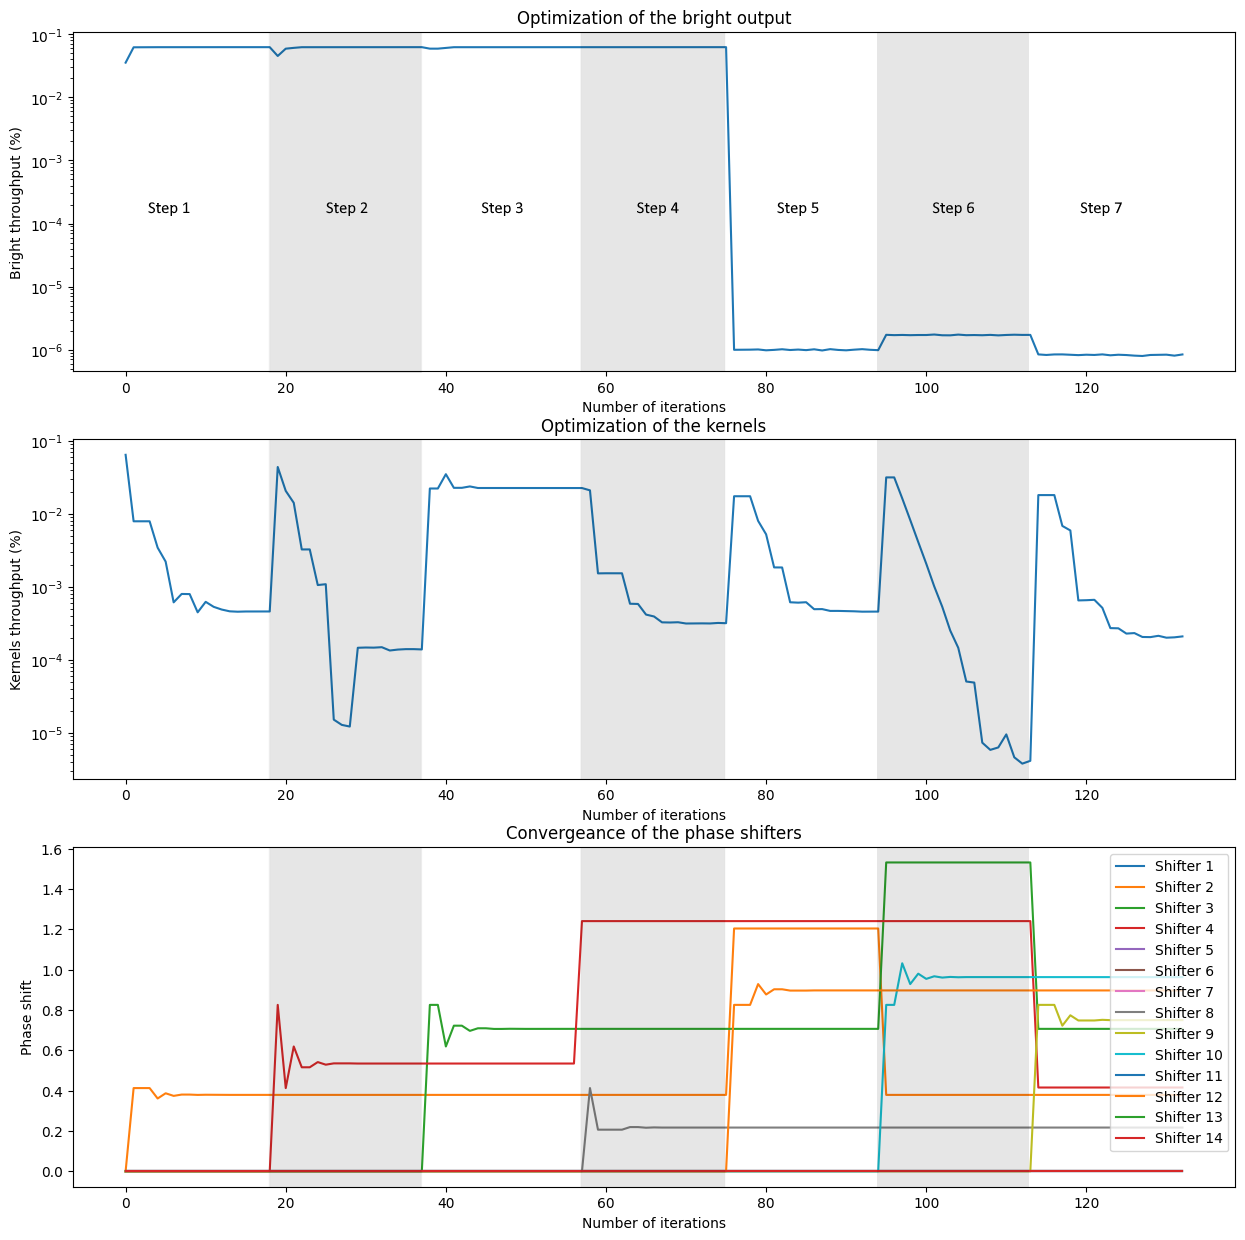
\includegraphics[height=7cm]{img/calibration_obstruction.png}
                \end{tabular}
                \end{center}
                \caption[calibration_obstruction] 
                { \label{fig:calibration_obstruction} 
                Calibration using input obstruction [AJOUTER DESCRIPTION]}
            \end{figure}

    \begin{figure}[H]
        \begin{center}
        \begin{tabular}{c}
        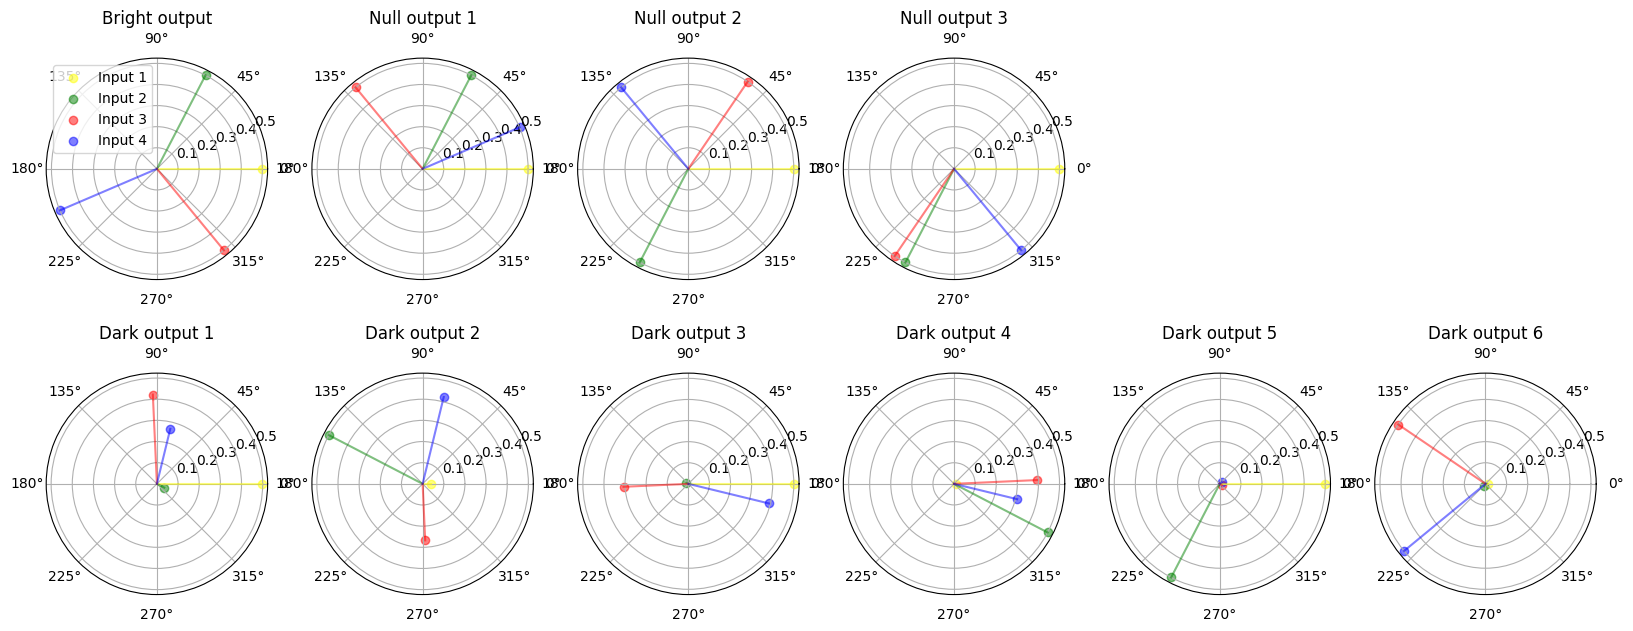
\includegraphics[height=3.2cm]{img/perturbed_phases.png}
        \end{tabular}
        \end{center}
        \caption[perturbed_phases] 
        { \label{fig:perturbed_phases} 
        Perturbed phases}
    \end{figure}

    \begin{figure}[H]
        \begin{center}
        \begin{tabular}{c}
        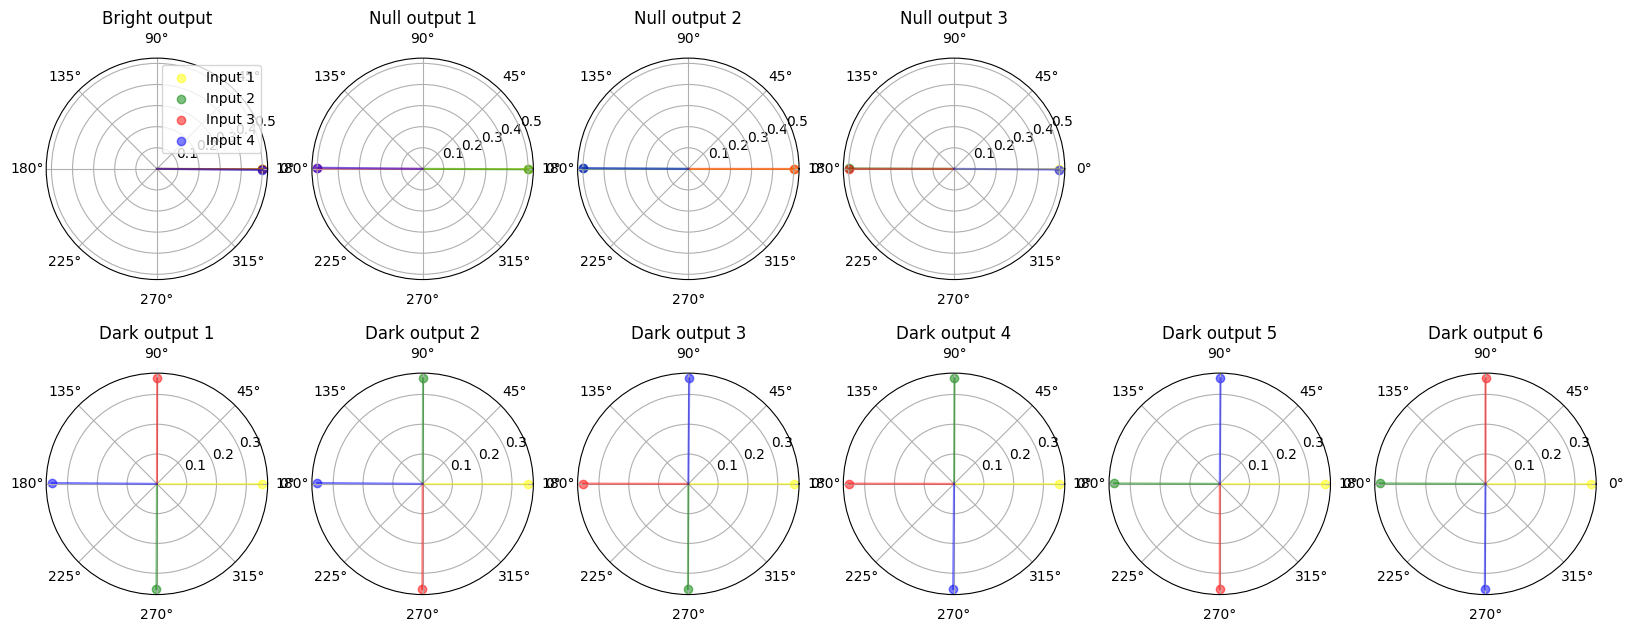
\includegraphics[height=3.2cm]{img/calibrated_phases.png}
        \end{tabular}
        \end{center}
        \caption[calibrated_phases] 
        { \label{fig:calibrated_phases} 
        Calibrated phases}
    \end{figure}

%--------------------------------------------------------------------

\section{Results and limitations}

    \begin{enumerate}
        \item Numerical results
        \subitem Kernel-Null depth (Fig \ref{fig:calibration_genetic} \& \ref{fig:calibration_obstruction})
        \subitem Kernel inversion and swapping 
        \item Laboratory results
        \item Laboratory limitations (ex. crosstalk)
    \end{enumerate}

    \begin{figure}[H]
        \begin{center}
        \begin{tabular}{c}
        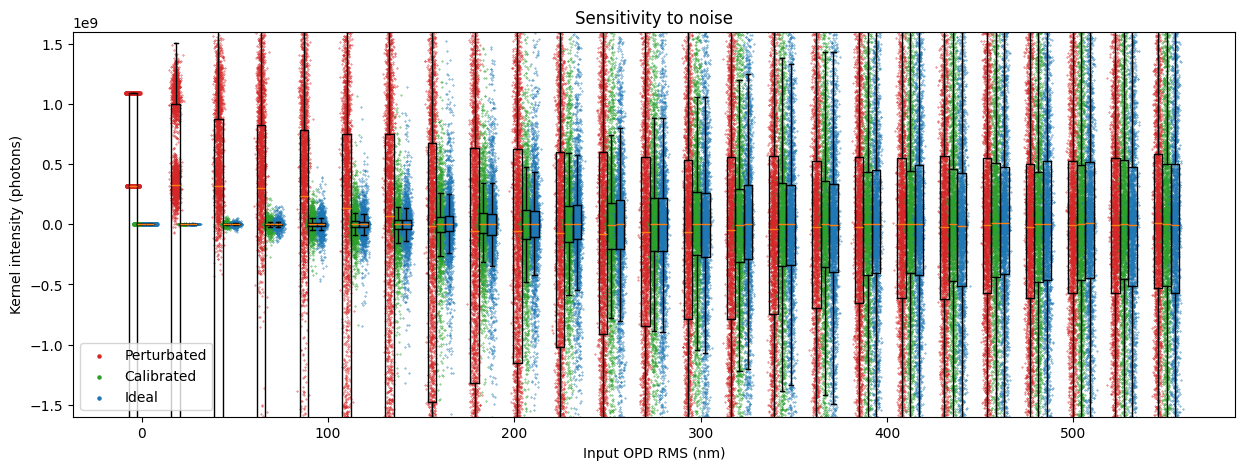
\includegraphics[height=3cm]{img/noise_sensitivity.png}
        \end{tabular}
        \end{center}
        \caption[noise_sensitivity] 
        { \label{fig:noise_sensitivity} 
        Sensitivity to input noise}
    \end{figure}

%-----------------------------------------------------------------

\section{Conclusions and prospects}

   \begin{enumerate}
      \item Conditions for noticing a performance gain
      \item Need of a post calibration caracterization process to identify the outputs
      \item Deeper statistical analysis is required to truely caracterize performance gain (the null depth is not the only relevant parameter)
      \item Architecture limitations (ex. no amplitude modulation, no photometric outputs)
   \end{enumerate}

\begin{acknowledgements}
      Lorem ipsum
\end{acknowledgements}

% WARNING
%-------------------------------------------------------------------
% Please note that we have included the references to the file aa.dem in
% order to compile it, but we ask you to:
%
% - use BibTeX with the regular commands:
%   \bibliographystyle{aa} % style aa.bst
%   \bibliography{Yourfile} % your references Yourfile.bib
%
% - join the .bib files when you upload your source files
%-------------------------------------------------------------------

\begin{thebibliography}{}

  \bibitem{lorem ipsum} Lorem ipsum

\end{thebibliography}

\end{document}
